\chapter{Background}
\lettrine[lines=4, loversize=-0.1, lraise=0.1]{T}{he following subsections} will address the background of speech recognition technology and requirement management. It will also indulge the reader in the background of Systemite AB, the company where this research and development of the system SpeechWeaver was conducted, as well as their application product line management software, SystemWeaver. Finally, it will give the reader an brief description of the Android Operating System and its history since its release in 2008.

\section{Speech Recognition}
Speech recognition as a technology has been available for a long time and can be traced back to an article by~\citet{davis1952} where they could recognize spoken telephone quality digits at normal speech rates by a single individual, having an accuracy varying between 97 and 99 percent. In the beginning of the history of software speech recognizers the computing power and algorithms were not good enough to give satisfying results. The speech recognizers have developed over the years to become more efficient and accurate. Recently, algorithms have started to run in parallel and sequentially to give better results. Furthermore the corpora have developed over the years to become more and more extensive~\citep{BakerJ}.

Since the introduction of smartphones, it is now an easy task to capture the users' speech in the phone and offload the speech recognition to cloud data centers. This makes speech recognition available anywhere the user might be when connected to the Internet. Speech recognition is also available offline with minor accuracy losses in the recognition capabilities \citep{androidIO2012}.

October 4, 2011 Apple included the intelligent personal assistant application "Siri" with the release of IOS5 and not long thereafter Google launched their equivalent on Android called "Google Now"~\citep{sirirelease,googlenowrelease}. These tools have made speech recognition available to the general public.

\section{Annotations}
Annotations are commonly used in software development to provide additional information in the source code and code development artifacts, e.g. constraint annotations (pre-/post conditions) in code or annotations to UML diagrams.
However, for other types of documentation, e.g. requirements and specification documents, annotation of individual entries is uncommon.
An example of such an annotation, i.e. an informal annotation, could be ``the test results need to go here'', which could serve as a reminder for future work or other additional information to clarify the entity.
However, most annotations consists of meta data that help simplify search and filter functionality, i.e. formal annotations.
Formal annotations are primarily intended to be read by machines, e.g. for Semantic-web applications~\citep{uren2006semantic}.
An example could be the annotation ``Paris'', which can be related to the abstract concept ``City'' or the country ``France'' given an ontology that helps reduce ambiguity of which ``Paris'' the annotation refers to. 
A considerable body of work has been devoted to formal annotation whilst lightweight informal annotations has been left an unexplored area.

\section{Requirement management}
Forward and Lethbridge conducted a survey in 2002 about Software Documentation~\citep{forward2002}. In the survey, they present that 54\% of the 32 participants thought that word processors was a useful documentation technology. In the same year, \citet{juristo2002european} wrote an article that presented that many organizations considered word processors to have an advantage in its simplicity for applications with few requirements. However, for those with more than 1000 requirements (approximately) , the disadvantages, such as scalability and no baseline, outweighed the advantages. Forward and Lethbridge also asked about how often the documentation was updated when changes occurred in the system, and they recipients answered that much of the design documents such as the SRS was rarely updated. The result from the question "How often is documentation updated when changes occur in a software System?" can be seen in Figure~\ref{fig:forward}. 

\begin{figure}[h]
\centering
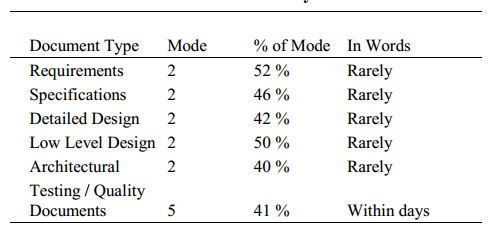
\includegraphics[width = 300pt, keepaspectratio = true]{fig/letforward2}
\caption{Results presented by Forward and Lethbridge about maintenance of documentation. The question asked was "How often is documentation updated when changes occur in a software System?"~\citep{forward2002}}
\label{fig:forward}
\end{figure}
\FloatBarrier

From the survey Forward and Lethbridge presents two suggestions:
\begin{quotation}
"Document content can be relevant even if it is not up to 
date. (However, keeping it up to date is still a good objective). As such, technologies should strive for easy to use, lightweight and disposable solutions for documentation."~\citep{forward2002}
\end{quotation}

and

\begin{quotation}
"Documentation is an important tool for communication and should always serve a purpose. Technologies should enable quick and efficient means to communicate ideas as opposed to providing strict validation and verification rules for building facts."~\citep{forward2002}.
\end{quotation}

Further support for the need of lightweight requirement practices is given by \citet{zhang2010towards} who discusses the importance of lightweight requirement processes in agile development. 
\citet{kauppinen2004implementing} claims that organizations can gain requirements engineering (RE) benefits by defining simple RE processes and focusing on a small set of RE practices, and by supporting the systematic usage of these practices.

Annotations are perceived to raise requirement quality and the use of annotations should therefore be integrated into the company's requirements engineering process


\subsection{Quality of requirements}
Guidelines for how to work with SRSs and how to work with software life-cycle processes has been developed by IEEE \citep{IEEE12207,IEEE830}. \citet{IEEE830} describes what characteristics that make a good SRS, in this way describing how to make high quality SRSs. \citet{IEEEtermin} defines quality as:
\begin{enumerate}
\item \textit{The degree to which a system, component, or process meets specified requirements.}
\item \textit{The degree to which a system, component, or process meets customer or user needs or expectations.}
\end{enumerate}

The first description defines quality of systems to which degree they meet the specified requirements, this means that if the specification is not up to date, and not clear enough, high quality can not be achieved, since it does not longer meet the specified requirements. This is however covered in the second description. If you look at the quality of an SRS, it should conform to the same two descriptions, but the requirements should conform to the software instead, i.e.\ the quality of an SRS should be to the degree it meets the \emph{actual, intended} functionality of the system as well as being precise and unambiguous. This gives that in order of a project to be of high quality, both these should be met to a high degree.

\section{Systemite AB}
\emph{Systemite AB} was founded in 2000 based of the recognition of problems with traditional (and often document based) processes in requirement management, configuration management and product data management. The three founders Anderson, Strömberg and Söderberg, all with experience from the automotive industry, developed a platform, \emph{SystemWeaver}, to gather all the design processes within an engineering organization into the same knowledge database. 

\section{SystemWeaver}
\label{sec:SystemWeaver}
SystemWeaver is a product line management software application developed by Systemite AB. 
It is an enterprise-wide data repository that assembles design information from all components of a software system, such as internal structure, interfaces, variants, versions, requirements and component status, in models \citep{systemiteStruct}. The models can be traversed and edited in a graphical interface, SystemWeaver Explorer. An abstract overview of SystemWeaver can be seen in Figure~\ref{fig:syswovervhej}.

\begin{figure}[h]
\centering
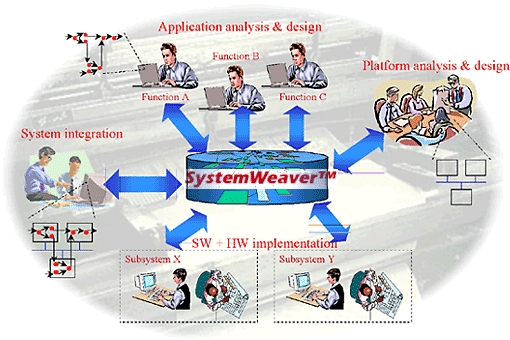
\includegraphics[width = 250pt, keepaspectratio = true]{fig/systemweaverbild}
\caption{An overview of \emph{SystemWeaver}}
\label{fig:syswovervhej}
\end{figure}
\FloatBarrier

\subsection{Parts \& Items}
The foundations of all of \emph{SystemWeaver's} models are \emph{items} and \emph{parts}. Items are the entities in the system, e.g. components, whilst the parts are the relationships between these entities. %EA: correct what I wrote? %O&V updaterat. Inte korrekt
An item or a part must be an object within a model, each with an unique identifier and a type identifier. 
The type identifier is called a SystemWeaver Identification (SID) that specifies the type of a model object.
For example, every object that has the SID 'RQQ' is a 'Generic requirement' whilst and object with the SID 'HWC' is a 'Hardware Component'. An example is a query based on 'Generic Requirement' items, with the subitems 'Functional Requirement' and 'Quality Requirement', that returns all of the items. This enables queries on specific levels at the same time as it makes it possible to aggregate data connected to items that are derived from the same type of items.

Parts, in turn, are as mentioned relationship between items. 
Parts always points in one direction and can define relationships such as 'Item A contains Item B' or 'Item A is derived from Item B'. The fact that the parts only points in one direction means that you would have to create two parts to make a two way relation.%EA: Do you need to define two parts to make a two way relation? Clarify.
%O&V: Har lagt till en bild. Ger den någon klarhet? 
The relationships an item can have to another item is within a model is defined by the meta model that was developed by Systemite AB's application engineers for the project.

\subsection{Meta-Models and Models}
\label{subsec:mmandm}
\emph{Systemite AB} are very flexible with their deployment of \emph{SystemWeaver} to their customers. This flexibility is made possible since all correlations and the behavior of items and parts are defined by a structured meta model that supports architectural and solution reuse as well as tailored solutions for specific customers.
Therefore, each project carried out in SystemWeaver is still unique but also very adaptable. 
Furthermore, because of the meta model solution, items and parts can look and behave in several different ways in different models dependent on what constrictions and rules the meta model has defined.

\subsection{Issues}
\label{subsec:issue}
SystemWeaver also supports task definition and tracking.
Tasks in SystemWeaver are called 'issues', and are, in a simple analogy, similar to notes that can be attached to items. 
Issues are used for case management of the items that they are attached to and can be set to different states, which are customizable in the meta-model (e.g. started, closed, assigned to). 
Issues can either point to items or other issues through an issue relation.
This relation can only be applied if the origin of the relation is an issue. Furthermore, similar to both items and parts, issues themselves all have SIDs. A graphical representation of how the artifacts in SystemWeaver fits together can be seen in Figure~\ref{fig:sysw}

SystemWeaver was used as a requirement database and backend in this project to facilitate the annotation scheme of SpeechWeaver.

\begin{figure}[h]
\centering
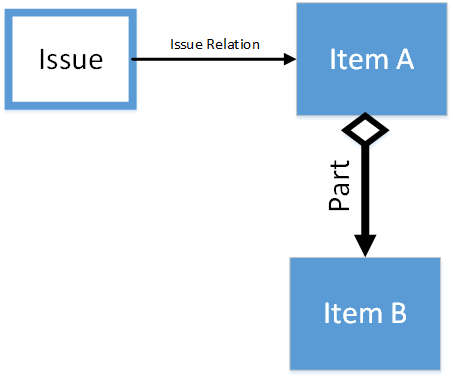
\includegraphics[width = 200pt, keepaspectratio = true]{fig/itemspartissuerelation}
\caption{A basic graphical representation of the correlations between the artifacts in SystemWeaver}
\label{fig:sysw}
\end{figure}


\subsection{SystemWeaver Report Generation}
Built into \emph{SystemWeaver} is an XML-based script language which allows for a user to generate reports based on information that can be gathered from the items and parts. The script language uses the parts to traverse through the item structure, and uses the items to collect information, e.g.\ present the title-field, creation date and description-field from all items of type ``RQQ" \citep{systemweaverHelpdoc}.

\section{Android Operating System}
The following section will give a background to the Android platform. We will briefly go through Android's history and development since its release give some background on the introduction of speech recognition in the platform.

\subsection{History}
Android is a Linux-based Operating System mainly focused on touch-devices such as tablets and smartphones. Android is Open Source and released under the Apache License 2.0~\citep{andlicense}.

Android was originally a product of Android Inc. In 2005, Google acquired Android Inc. and began to develop the platform \citep{androidAquire}. Google reached out to several different companies, working with hardware, handset and networks, to form the Open Handset Alliance which was announced in 2007~\citep{openhandsetalliance}. The alliance works for advancing open standards for smart phones, tablets and other mobile smart devices. In 2008 the first phone running Android~1.0 was released~\citep{helalBose,andrelease}. 

Android developed and refined the Operating System and released several updates and versions over the upcoming years. In November 2012, version 4.2 (code name Jelly Bean) was released. By then, Android had become the most popular mobile platform with over 600.000 applications and games available for the platform, and over 400.000.000 activated Android devices~\citep{androidhome}.

\subsection{Speech Recognition in Android}
Along with the release of version 2.1 (code name Eclair), Android included a speech-input feature to their keyboard. The featured allowed for users to dictate messages with their speech instead of typing them with their fingers. The distribution of Android devices capable of running speech recognition is about 99.9\% as can be seen in Table~\ref{tab:anddist} \citep{andspeechrec}. 
\begin{table}[h]
\centering
\caption{Android Platform version distribution (Data collected during a 14-day period ending on April 2, 2013)\citep{andDist}}
    \begin{tabular}{ l  l  l  l }
        \hline
        Version & Codename & API & Distribution \\
        \hline 
        1.6 & Donut & 4 & 0.1\% \\ 
        2.1 & Eclair & 7 & 1.7\% \\
        2.2	& Froyo & 8 & 4.0\% \\
        2.3 - 2.3.2 & Gingerbread & 9 & 0.1\% \\ 
        2.3.3 - 2.3.7 &	Gingerbread & 10 & 39.7\% \\ 
        3.2 & Honeycomb & 13 & 0.2\% \\
        4.0.3 - 4.0.4 &	Ice Cream Sandwich & 15 & 29.3\% \\ 
        4.1.x &	Jelly Bean & 16 & 23.0\% \\
        4.2.x & Jelly Bean & 17 & 2.0\% \\ 
        \end{tabular}     
\label{tab:anddist}
\end{table}























